%
% Since this is a ``report'', the topmost level of hierarchy is
% ``Chapter'', not section as you may be used to. Chapters are
% enumerated starting from 1, so Sections are 1.1, Subsections are
% 1.1.1, subsubsections don't get numbers. (You can change that, if
% you want them to be called 1.1.1.1)
%
\chapter{Policy Inference with Gaussian Policy Estimate}\label{chapt:gauss_policy}

    The multi-agent system presented in this thesis is modeled with two agents, the controllable agent \agent{1} and the
    uncontrollable agent \agent{2}. Explicitly, these agents exist within a hidden-parameter \ac{MDP}, where the hidden
    parameter is the action distribution, policy, of \agent{2}. If \agent{1} is given a task, it can only robustly plan
    for this task when it has an accurate estimate of how \agent{2} will act. Determining the action distribution of an
    uncontrollable agent given its current state is known as \textit{policy-inference}. The following definitions
    present a formal definition of a hidden policy in \iac{MDP}, but Chapter \ref{chapt:policy_iteration} will discuss
    methods of actually solving for policies.

    After defining the hidden-parameter MDP, this chapter presents an inference method that uses Monte-Carlo integration
    of policy parameters sampled from a multivariate distribution. This algorithm is independent of the actual policy
    parameterization, which will then be presented in Section \ref{sec:policy_parameterization}.  Finally, the algorithm
    will be tested in a single-agent grid world before demonstrating a two agent example in Chapter
    \ref{chapt:proactive_inference}. We could extend the number controllable and uncontrollable agents but a two agent
    example sufficiently demonstrates the algorithm framework.



\section{Hidden-parameter MDP}\label{sec:hipmdp}
    \begin{definition}
        The interaction between two agents is captured by an hidden-parameter \ac{MDP},
        \[
            M = (S, A_1 \times A_2, R, T, \policy{2}, I , \gamma)
        \]
        with the tuple defined as in \cite{Sugiyama2015StatisticalRL} plus the hidden parameter, $\policy{2}$:
        \begin{itemize}
                \item $S \equiv (S_1 \times S_2)$ is a set of joint states with cardinality $0 < |S| \leq \infty$ .
            \item $A_1\times A_2$ is a finite set of actions, where $A_1$ is the set \agent{1} can execute and $A_2$ is
                the set available to \agent{2}.
            \item $R: S\times A_1 \rightarrow \reals$ is the real-valued state-action reward function given to the
                controllable agent.
            \item $T: S\times (A_1\times A_2)\rightarrow \dist(S)$ is the probabilistic state transition function
                $ T(s'| s, (a_1,a_2)) $ which yields the probability of reaching state $\textnormal{s}'$ after both
                agents take action pair $(\text{a}_1,\text{a}_2)$ at the state $\textnormal{s}$.
            \item $\policy{2} : S \rightarrow \dist(A_2)$ The distribution of \agent{2}'s actions given a
                state. The probability of each action is $\policy{2}(a_2|s),\ \forall\ a_2 \in A_2$.
            \item $I \in \dist(S)$ is the initial state distribution.
            \item $\gamma$ The discounting factor $(0,1)$.
        \end{itemize}
    \end{definition}

    \noindent
    This definition also leads us to a couple pivotal assumptions in this work:

    \begin{assumption}
        The state-action transition function $P(\cdot)$, is known.
    \end{assumption}

    \begin{assumption}
        The unknown policy of \agent{2}, $\policy{2}$, produces a stationary- and ergodic-stochastic process; the policy
        is Markovian.
    \end{assumption}

    Given that \agent{1} takes some action $a_1$, the distribution of next states is

    \begin{equation}\label{eq:true_state_action_trans_prob}
        P(s'| s, a_1) = \sum_{a_2\in A_2} T\left(s'|s, (a_1,a_2)\right)\policy{2}(a_2|s).
    \end{equation}

    \noindent
    With this model, the true probability of a future state $s'$ given the current state $s$ is

    \begin{equation}\label{eq:true_state_trans_prob}
        P(s'|s) = \sum_{a_1, a_2 \in A} T \left(s'|s, (a_1,a_2)\right)\policy{2}(a_2|s)\policy{1}(a_1|s),
    \end{equation}

    \noindent
    where, for simplicity, this report uses identical action sets, $A_1 \equiv A_2 \equiv A$. Methods to obtain
    (sub)optimal policies for the controllable agent, $\policy{1}$, will be discussed in Chapter
    \ref{chapt:policy_iteration}. Finally, the \ac{MDP} formed by the tuple $(S, A_1 \times A_2, R, T, \policy{2}, I ,
    \gamma)$ will be referred to as $\mathcal{M}$. Let's now justify the algorithm used for policy inference.

    \todo[inline]{Potentially explain the difference between HIP-MDP and POMDP?  }


\section{Policy Inference Objective Function}\label{sec:policy_obj}
    Consider that the main goal of \agent{1} is to complete its task and a secondary goal is to infer the policy of
    \agent{2}. The estimate of \agent{2}'s policy, $\estimate{\policy{}}_2$, is parameterized by a vector \vect{\theta}.
    Therefore, the estimated probability of a state transition is

    \begin{equation}\label{eq:est_state_trans_prob}
        q(s'|s, \vect{\theta}) = \
            \sum_{a_1, a2 \in A}P(s'|s,(a_1,a_2))\estimate{\policy{}}_2(a_2|s,\vect{\theta})\policy{1}(a_1|s).
    \end{equation}

    As the \agent{2} moves through $S$, the robot agent can observe the outcomes of \agent{2}'s actions, and build a set
    of observed state sequences.

    \begin{definition}\label{def:traj}
            A trajectory $\tau$ is a sequence of joint states $s=(s_1, s_2)$ with time-step index $t$,
            \[
            s^{(0)}, s^{(1)}, \ldots , s^{(t)}, \ldots , s^{(|\tau|)};\ 0 \leq t \leq |\tau|.
            \]
    \end{definition}

    We'll define the probability of a trajectory as the joint probability of each set state-transition tuple for each of
    the two distributions, $p$ and $q$:

    \begin{align*}
            p(\tau) &= \prod_{t=1}^{|\tau|}p\left( s^{(t)}| s^{(t-1)} \right), \\
            q(\tau|\vect{\theta}) &= \prod_{t=1}^{|\tau|}q\left(s^{(t)}| s^{(t-1)}, \vect{\theta}\right).
    \end{align*}

    \noindent
    By using the parameter \paramVec, $q(\tau,\paramVec)$ is the probability of replicating a trajectory given the
    parameterization. We'll sample a set of trajectories and build an observed demonstration set, $\tau_d \in D$.

    \begin{assumption}
        The observed demonstration set, D, is sampled i.i.d. from the set of all possible demonstrations $\mathcal{D}$.
    \end{assumption}

    The best inference of an environmental policy has a high likelihood of replicating the trajectories in $D$.
    \begin{lemma}\label{lemma:obj_fun_equiv}
        Minimizing the \ac{KLD} of the replica distribution from the observed trajectory distribution is equivalent to
        maximizing the log-likelihood of the observed state sequences given a parameterized policy, With a fixed policy
        for \agent{1}, $\policy{1}$,

        \begin{equation*}
            \argmax_{\paramVec} \logLike(\paramVec; \policy{1}) = \argmin_{\paramVec} \text{KL}(p||q_{\paramVec}).
        \end{equation*}
    \end{lemma}

    \begin{proof}
        Consider a pair of stationary policies for the two agents, $\policy{1}$ and $\policy{2}$. The induced Markov
        chain is $M_{\policy{1}, \policy{2}}$. Let $p$ be the probability distribution of paths in the chain
        $M_{\policy{1}, \policy{2}}$. Let $q_{\paramVec}$ be the probability distribution of paths in the chain
        $M_{\policy{1}, \estimate{\policy{}}_2}$. The \ac{KLD} from $q_{\paramVec}$ to $p$ is

        \begin{equation*}\label{eq:traj_kl_div}
            \text{KL}(p || q_{\paramVec}) = \sum_{\traj_d \in D} p(\traj_d) \ln \left( \frac{p(\traj_d)}
                                                {q(\traj_d|\paramVec)} \right)\
                = \sum_{\traj_d \in \calD} P(\traj_d|D) \ln \left( \frac{P(\traj_d|\calD)}
                                                {P(\traj_d|\policy{1},\paramVec)} \right),
        \end{equation*}

        \noindent
        where $P(\traj_d|D)$ is the maximum likelihood probability of the state sequence, and
        $P(\traj_d|\policy{1},\paramVec)$ is the probability of obtaining that state sequence by our inferred policy
        that is parameterized by the vector \paramVec.

        Minimizing the deviation of $q_{\paramVec}$ from $p$ is equivalent to maximizing the expectation of the
        observing $D$, given that the environment actions are distributed as $\policy{2}(s; \paramVec)$:

        \begin{equation}\label{eq:min_kld}
            \begin{aligned}
                \argmin_{\paramVec}(\text{KL}(p || q)) & = \
                    \argmin_{\paramVec}\left(\sum_{\traj_d \in  \calD}\!  P(\traj_d|\calD)
                    \ln\left(\frac{P(\traj_d|\calD)}{P(\traj_d|\policy{1},\paramVec)}\right)\right)\\
                & = \argmin_{\paramVec}\left(\sum_{\traj_d \in D} P(\traj_d|D) \ln(P(\traj_d|D)) -
                    P(\traj_d|D) \ln\left(P(\traj_d|\policy{1},\paramVec)\right)\right)\\
                & = \argmax_{\paramVec}\left(\sum_{\traj_d \in \calD}\!  P(\traj_d|\calD)
                    \ln\left(P(\traj_d|\policy{1},\paramVec)\right)\right)\\
                & = \argmax_{\paramVec}\expectation{P(\traj_d|\calD)} {\ln(P(\traj_d|\policy{1},\paramVec))} \\
                &\approx \argmax_{\paramVec} \sum_{\traj_d \in D}  \ln(P(\traj_d|\policy{1},\paramVec))\\
                & =\argmax_{\paramVec} \logLike(D|\policy{1},\paramVec)
            \end{aligned}
        \end{equation}

        \noindent
        where we estimate the expectation using the empirical mean. We will write the final line of Eq.
        \ref{eq:min_kld} as $\logLike(\paramVec; \policy{1})$ for compactness and consistency with Lemma
        \ref{lemma:obj_fun_equiv}.

    \end{proof}

    For the rest of this report, lets assert that an optimal parameter exists.
    \begin{assumption}\label{assump:opt_policy_err}
        There exists an optimal parameter vector that can represent the true distribution of $\policy{2}(s)$ to within a
        threshold $\xi$, given that a set of basis functions are properly defined;
        \[
        \exists\ \optimal{\paramVec}\ \big|\ \Big| \OneNorm{\estimate{\policy{}}_2(s;\optimal{\paramVec})} -
            \OneNorm{\policy{2}(s)} \Big| \leq \xi.
        \]
    \end{assumption}

    \noindent
    The $\mathsf{L_1}$-norm of a policy, $\OneNorm{\policy{}(s)} = \sum_{s \in S}\sum_{a \in A}\policy{}(a|s)$, is a
    measurable distance unlike \ac{KLD}; $\text{KL}(p||q) \neq \text{KL}(q||p)$. For all following experiments, we'll
    use the absolute difference of $\mathsf{L_1}$-norm's to compare two policies.

    We are now ready to discuss the inference procedure used to identify the $\estimate{\policy{}}_2(s,
    \estimate{\paramVec})$ that maximizes the R.H.S of Lemma \ref{lemma:obj_fun_equiv}.

\subsection{Gaussian Distribution of Policy Parameters}\label{sec:gauss_policy}

    \todo[inline]{This should probably be moved to Chapter 4. Need a simpler explanation in this
                  section-introduction.}

    Assuming that \agent{1} has received some initial data $D^{(0)}$, the estimated policy of the uncontrollable agent
    can be improved from some initial guess $\estimate{\policy{}}_2^{(0)}$. To prepare for active inference in Chapter
    \ref{chapt:proactive_inference}, let's assume that $D^{(0)}$ could be incomplete. It might not contain enough data
    for the following algorithm to meet the tolerance required by Assumption \ref{assump:opt_policy_err}. Therefore,
    \agent{1} will need to gather more data, trajectories, $D^{(b)},\ b=1,\ldots,B$. Ideally, $D^{(b)}$ will contain
    data that was lacking in all previous batches. When there is not enough data, some estimates parameter elements,
    $\estimate{\theta}_\paramIdx$, will be incorrect. The algorithm needs to quantify an uncertainty metric to guide
    data collection, and improve any parameter elements with high uncertainties.

    First, let's only consider one batch of data, so the estimated parameter vector in the $b$-th batch,
    $\estimate{\paramVec}^{(b)}$ can simply be represented as \estimate{\paramVec} for the rest of this section. Then,
    let $\estimate{\paramVec} = [ \paramElem]_{w=1}^W$ be a vector of independently sampled random variables with
    distributions $\mathcal{N}(\mu_w, \nu_w)$. The variance, $\nu_w^2$ will capture the uncertainty of \paramElem in the
    inference from dataset $D$.

    We denote $\rho_w = (\mu_w, \nu_w)$ the tuple of mean and variance for $\paramElem$ and denote $\rho
    =\{\rho_w\}_{w=1}^W$ to be the collection of variable tuples.  Given $\rho$, the probability of the demonstrations
    is
    \[
    P(D |\rho) = \int_{\paramVec } P(D|\paramVec) p(\paramVec | \rho)d\paramVec.
    \]

    \noindent
     The log-likelihood of the demonstrations can be lower-bounded using Jensen's inequality:
    \begin{equation*}
    \logLike(D|\vect{\rho} ) = \log P(D|\rho)\
         = \log \left( \int_{\theta}P(D|\theta) p(\theta | \rho)d\theta \right)\
         \ge \int_\theta p(\theta|\rho)\log \big( P(D|\theta) \big) d\theta.
    \end{equation*}


    Denote this lower bound as $\tilde{\logLike}(D|\rho)=\int_{\paramVec} p(\paramVec |\rho) \log P(D|\paramVec)
    d\paramVec$. This is the lower bound on the objective function derived in Eq. \ref{eq:min_kld}!  By taking
    derivative of $\tilde{\logLike}(D|\rho)$ with respect to $\rho$, we obtain the gradient of the objective function:
    \begin{equation}\label{eq:logLike}
        \begin{aligned}
            \nabla_\rho \tilde{\logLike}(D|\rho)) & =
                \int_{\paramVec}\nabla_\rho p(\paramVec|\rho) \log P(D|\paramVec)d\paramVec\\
            & = \int_{\paramVec}[ p(\paramVec|\rho) \nabla_\rho \log p(\paramVec|\rho) ] \log P(D|\paramVec)d\paramVec\\
            &\approx \frac{1}{m} \sum_{ i=1}^m \left[\nabla_\rho \log P(\paramVec^{(i)}|\rho) \right] \log
                P(D|\paramVec^{(i)})
        \end{aligned}
    \end{equation}

    \noindent
    where $\paramVec^{(i)}$, $i=1,\ldots, m$ are samples generated from the multi-variant Gaussian distribution with
    mean  $\vect{\mu} = [\mu_1,\ldots, \mu_W]^\top$ and covariance matrix $\mbox{diag}\left(\nu_1,\ldots, \nu_W\right)$.
    Let $\vect{\nu}$ be an equivalent representation for $\mbox{diag}\left(\nu_1,\ldots, \nu_W\right)$. Each sampled
    parameter element, $\paramElem^{(i)}$ has probability:

    \[
        P(\paramElem^{(i)} | \rho_{\paramIdx}) =  \frac{1}{\sqrt[]{2\pi \sigma_w^2}}\exp \left( -
        \frac{(\theta_w^{(i)}-\mu_w)^2}{2\sigma_w^2} \right).
    \]

    The bracketed gradient in the last line of Eq. \ref{eq:logLike} with respect to each element of \vect{\mu} and
    $\vect{\nu}$ are:
    \[
    \nabla_{\mu_{\paramIdx}}\log P(\paramElem^{(i)} | \rho_{\paramIdx}) =
        \frac{\paramElem^{(i)} - \mu_{\paramIdx}}{\nu_{\paramIdx}^2},\ \text{and}
    \]
    \[
    \nabla_{\nu_{\paramIdx}}\log P(\paramElem^{(i)} | \rho_{\paramIdx}) = \frac{(\paramElem^{(i)} - \mu_{\paramIdx})^2 -
        \nu_{\paramIdx}^2}{\nu_{\paramIdx}^3}.
    \]
    Note that superscripts enclosed in parenthesis represent sample indexes, e.g., the $i$-th sample of parameter
    element $w$ is $\paramElem^{(i)}$. All purely numeric superscripts are exponents.


    We can obtain the optimal collection of parameters $\optimal{\rho}= \argmax_{\rho} \tilde{\logLike{}}(D|\rho)$ by
    performing gradient ascent on the parameter distributions, $\rho = (\vect{\mu}, \vect{\nu})$. The policy
    parameterized by $\optimal{\estimate{\paramVec}} \sim \mathcal{N}(\optimal{\vect{\mu}}, \optimal{\vect{\nu}})$ is
    $\estimate{\policy{}}_{2}(s; \optimal{\estimate{\paramVec}})$ and it maximizes the log likelihood of the
    demonstration set $D$. The log likelihood of observed demonstrations for a given $\paramVec^{(i)}$ can be computed
    as
    \begin{align*}
        \log P(D|\paramVec^{(i)}) & = \sum_{\tau_d \in D} \log P(\tau_d |\paramVec^{(i)})\\
        & = \sum_{d=1}^{\abs{D}} \left[ \sum_{t=0}^{\abs{\tau_d}-1} \log P(s^{t+1}|s^t,(a_1, o_2^t)) +
            \sum_{t=0}^{\abs{\tau_d}-1}  \log \policy{2}(o_2^t|s^t; \paramVec^{(i)}) \right]\\
        & = \sum_{s\in S}\sum_{o_2\in A} C(s, o_2)  \log \policy{2}(o_2|s; \paramVec^{(i)}) + Const.
            \end{align*}
    \todo[inline, color=green]{Note the change between this equation and the CDC draft. I have dropped $a_1$ from $C(\cdot)$}
    Above, $C(s, o_2)$ is the number of times the state action pair $(s,o_2)$ is observed from in $D$, and
    $Const =\sum_{d=1}^{\abs{D}} \sum_{t=0}^{\abs{\tau_d}-1} \log P(s^{t+1}|s^t,(a_1^t,o_2^t))$, which is independent of
    $\paramVec^{(i)}$; the constant term and can be precomputed for a demonstration $D$. The observed action outcome at
    time-step $t$ is $o_2^t$, which is the only action information available in a trajectory, per Definition
    \ref{def:traj}.  If a trajectory fragment $(s_1, s_2)^{(t)}, (s_1', s_2')^{(t+1)}$ is observed, the action of the
    controllable agent $a_1^t$ is known but the uncontrolled action, $a_2^t$, is not.  Therefore $o_2^t$ is assigned to
    be the nominal motion that causes the transition $s_2^{(t)} \rightarrow s_2^{(t+1)}$ in the graph of $\mathcal{M}$.

    \todo[inline]{talk to Prof. Fu about the remark, below. I'm not automatically dropping basis functions, it would be
    hard to define that for only a single action at a kernel, but I could mask the parameter value to always be zero. }
    \begin{remark}
    If the policy does not depend on a basis function $\phi_k$, then the mean $\mu_k=0$ and the basis function will be
    removed from the set of basis function  as well as the corresponding parameter $\eta_i$. The inference algorithm is
    terminated based on relative tolerance rule:  in two consecutive update of $\rho$, the improvement in the  objective
    function drops below a given threshold.  \end{remark}

    \todo[inline]{describe moving average termination}


\subsection{Q-function Approximation}\label{sec:policy_parameterization}
    The model of $\policy{2}(s; \paramVec)$ approximates the \textit{state-action value function}, $Q(s,a_2)$, with a
    linear-in-parameter model. Sugiyama describes this model in detail in Section 2.2.1 of
    \cite{Sugiyama2015StatisticalRL}. It is advantageous that \agent{1} does not need to learn the reward function of
    \agent{2}, but only the distribution of \agent{2}'s action given the joint state $(s_1, s_2)$. Each parameter
    element determines the weighting of a feature $\phi : S \times A_2 \rightarrow \reals$. If a total of $\paramLen$
    features are used then \agent{2}'s Q-function is approximated as

    \begin{equation*}\label{eq:QFuncApprox}
        Q(s,a_2) \approx \estimate{Q}(s,a_2) = \sum_{\paramIdx=1}^{\paramLen} \estParamElem \featElem(s,a_2)
            = \estimate{\paramVec}^\top \featFunc.
    \end{equation*}

    Following Chapter 3 of \cite{Sugiyama2015StatisticalRL}, we'll use \acp{GGK} because they intuitively incorporate
    obstacles into a distance metric between a state $s$, and the center of a \ac{GGK}, $c$. Consider the state-graph of
    $\mathcal{M}$. If there are $K$ kernels, and the $l$-th kernel has center $c$, then the value of the kernel at a
    state $s$ is

    \begin{equation*}
        \kernFunc(s,\kernCent_{\kernIdx}) = \exp \left( \frac{-\text{SP}(s,\kernCent_{\kernIdx})^2}
            {2\kernStdDev^2_{\kernIdx}} \right).
    \end{equation*}

    \noindent
    The \ac{SP} between a state $s$ and the $l$-th kernel's center $c_l$ can be precomputed, and the kernel standard
    deviation, $\kernStdDev_{\kernIdx}$, determines an area-of-influence.  The feature function is defined for each
    action, so the number of features is $W = |A| \times K$. The $w$-th feature function is

    \begin{equation}\label{eq:kernel_func}
        \featElem(s_2,a_2) =I(a_2==a_2^{j})\sum_{s_2'\in S_2}P(s_2'|s_2,a_2^{j}) \kernFunc(s_2',c_{\kernIdx}),
    \end{equation}

    \noindent
    where $w=j+(\kernIdx|A_2|-1)$ represents the index used for both feature-vector functions and parameter elements,
    \paramElem.  Also, for each action $a_2$ the indicator function ${I(a_2==a_2^j)}$ is defined as:
    \begin{equation*}
        \begin{aligned}
            I(a_2==a_2^j) & = \begin{cases}
                                  0 & \text{if}\ a_2 \neq a_2^j \\
                                  1 & \text{if}\ a_2 = a_2^j
                              \end{cases} \\
            j & = 1, \ldots, |A_2|,
        \end{aligned}
    \end{equation*}

    \noindent
    assuming all actions are enabled from each state $s_2 \in S_2$.


    Given a $Q$-function, the policy at a state is represented as the softmax (Boltzman) over all actions,
    \[
    \policy{2}(a_2|s) \propto \exp(Q(s,a_2)/\kappa)
    \]
    where $\kappa$ is a temperature parameter. If $\kappa \rightarrow \infty$, the distribution $ \policy{2}(s) $
    becomes uniform over $A_2$. If $\kappa \rightarrow 0$, the distribution $ \policy{2}(s) $   becomes a Dirac Delta
    distribution that peaks on the action $a_2^\ast = \argmax_{a_2} Q(s,a_2)$. In the inference algorithm, we consider
    $\kappa$ as a predefined hyper-parameter in the range $(0,\infty)$.

    \todo[inline]{currently set to 1}

    According to \cite{nachum2017bridging}, the policy is also represented as
    \[
    \policy{2}(a_2|s) = \exp((Q(s,a_2)- V(s))/\kappa),
    \]
    where $V(s) = \log \sum_{a_2\in A}\exp (Q(s,a)/\kappa)$. This is the model used for \policy{2} in the rest of this
    report.  Again, the policy obtained with a $Q$-function parameterized by $\paramVec$ is denoted
    $\policy{2}(s;\paramVec) : S\rightarrow \dist(A)$.

\section{Single-agent policy inference experiment}
    The algorithm and parameterization presented in Sections \ref{sec:gauss_policy}-\ref{sec:policy_parameterization}
    are initially tested in a single agent environment. In this example, the states are just $s=s_2 \in S$, and
    $\policy{1}(a_1|s)$ is dropped from Eq. \ref{eq:true_state_trans_prob}.

    \subsubsection{Simulation environment}
    Assume that \agent{2} exists alone in a $5\times5$ grid world. The boarder of the grid-world are considered to be
    walls.

    \begin{table}[h!]
    \centering
    \begin{tabular}{ c || c | c | c | c}
              & \multicolumn{4}{|c}{Starting grid-cell location type}\\
        \hline
        Resulting Motion & Middle & Right Column & Top Row & Upper Right Corner\\
        \hline
        %      &       &       &       \\
        North & $0.1$ & $0.1$ & $0.0$ & $0.0$ \\
        South & $0.1$ & $0.1$ & $0.1$ & $0.1$ \\
        East  & $0.8$ & $0.0$ & $0.8$ & $0.0$ \\
        West  & $0.0$ & $0.0$ & $0.0$ & $0.0$ \\
        Stay  & $0.0$ & $0.8$ & $0.1$ & $0.9$ \\
    \end{tabular}
    \label{table:motion_model}
    \caption{Agent motion model given attempted \textit{East} (right) action.}
    \end{table}

    The \textit{hidden} policy of \agent{2} is visualized in Fig. \ref{fig:single_agent_2_policy}. The policy is
    deterministic, $\kappa=0$, and the agent has a hidden goal of the green cell. .... to-be-continued

    \todo[inline]{change the color of agent \textbf{2}'s goal to yellow, to limit confusion in future sections}

    \begin{figure}[htb]
        \begin{center}
            \fbox{
                \begin{minipage}{0.5\textwidth}
                    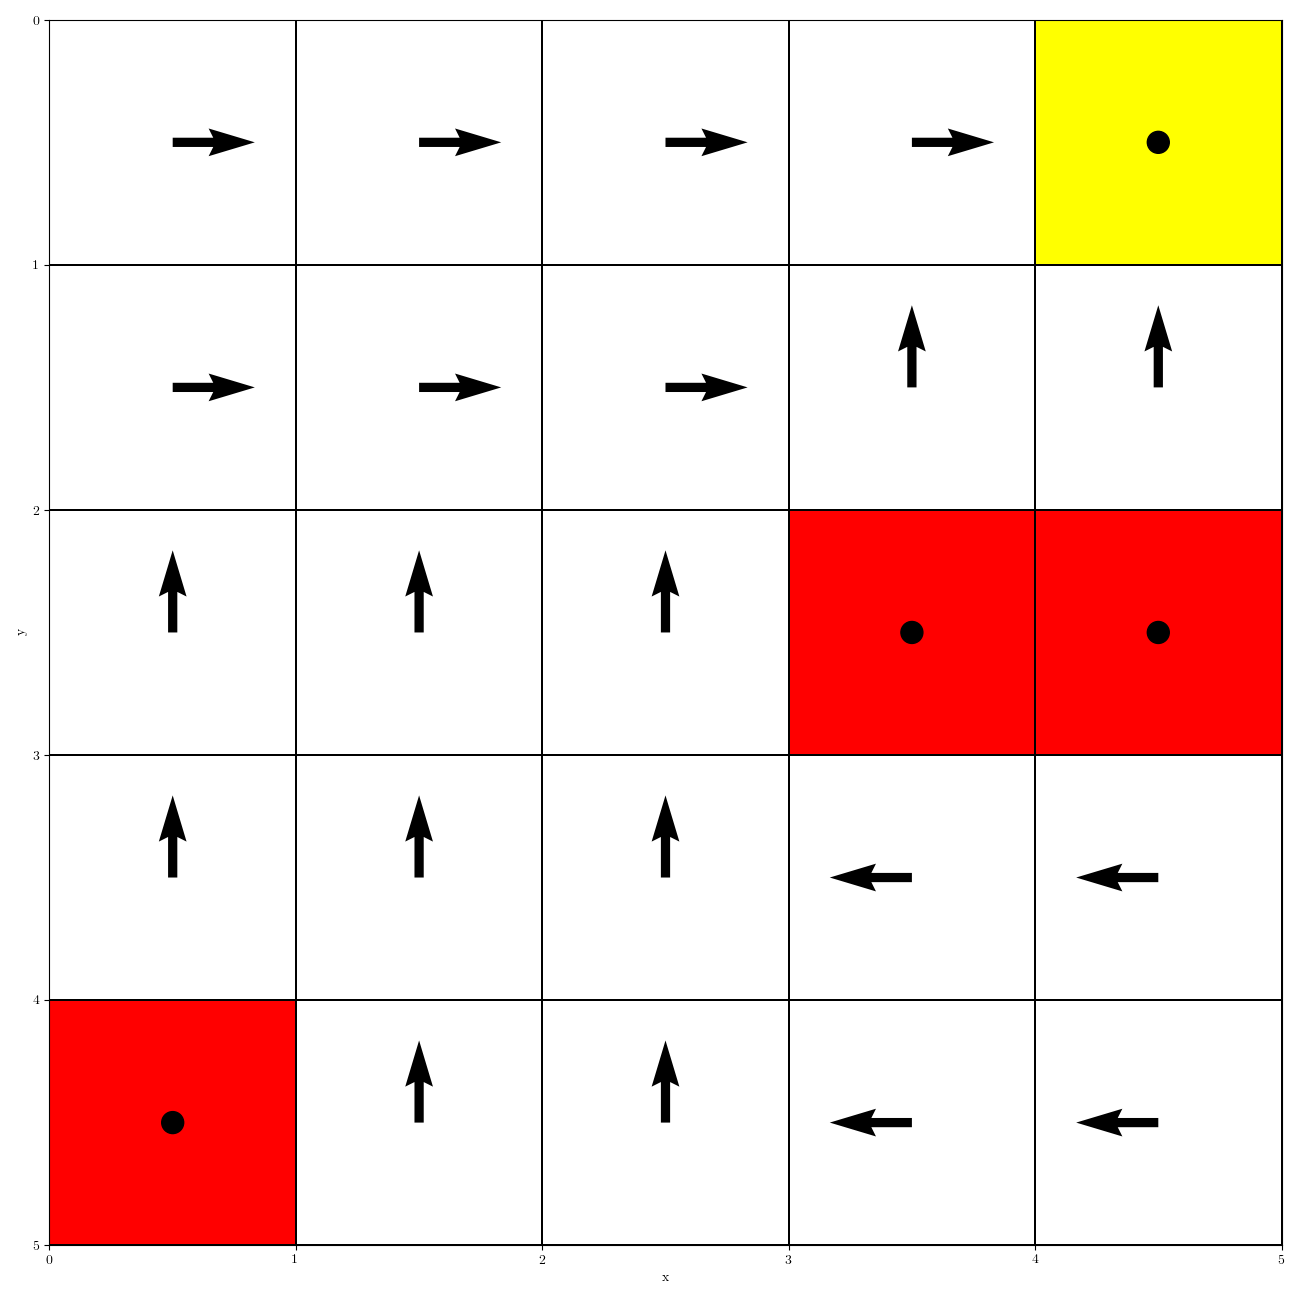
\includegraphics[width=\textwidth]{single_agent_2_policy}
                    \caption{Policy of \agent{2}.}
                    \label{fig:single_agent_2_policy}
                \end{minipage}
                }
        \end{center}
    \end{figure}
